% Requires graphicx, booktabs, references.bib; paths assume this directory.
\section{Experimental Validation and Analysis}
\label{sec:eval}
We evaluate a literature-parameterized nominal processor with two linked
protocols: swapping at R creates an A--B pair, and teleportation at A
consumes that same pair. Q2NS retains the classical protocol and real
packet path; NetSquid owns the quantum state and timed instruction chain.
% Requires booktabs and references.bib. All figures use this profile.
\paragraph{Literature-parameterized physical model.}
We adopt the nominal instruction times reported by Liao et al.\ in
\emph{Benchmarking of quantum protocols}~\cite{liao2022benchmarking}
(Table~3), and the matching H/X/Z, memory and gate-noise parameters
used by Iqbal et al.\ in \emph{Investigating Imperfect Cloning for
Extending Quantum Communication Capabilities}~\cite{iqbal2023cloning}
(Table~3 and Section~4).
\begin{table}[t]
\centering
\caption{Adopted nominal processor profile. Times and noise parameters are
from~\cite{iqbal2023cloning}; instruction times also appear
in~\cite{liao2022benchmarking}. Derived circuit durations are QuCl choices.}
\label{tab:qucl-physical-profile}
\small
\begin{tabular}{@{}lr@{}}
\toprule
Parameter & Value \\
\midrule
CNOT & 20~$\mu$s \\
H / X / Z & 5~ns each \\
Single measurement & 3.7~$\mu$s \\
Memory $T_1$, $T_2$ & 10~h, 1~s \\
Gate depolarization parameter $p$ & 0.01 \\
\midrule
Serial CNOT--H--M--M & 27.405~$\mu$s \\
Two correction slots & 10~ns \\
\bottomrule
\end{tabular}
\end{table}

NetSquid executes the timed instructions and applies native T1/T2 storage
noise. We explicitly implement the quoted gate parameter as independent
per-participating-qubit depolarization,
$\mathcal{D}_p(\rho)=(1-p)\rho+pI/2$, before each actual CNOT, H, X or Z,
after storage noise for the instruction's duration. The channel extends
locally to entangled qubits. Ideal measurements and unused identity
correction slots receive storage noise only. Both correction slots
reserve 5~ns regardless of the measured branch.
This noise placement and the serial measurement schedule are explicit
QuCl modeling choices, not an assertion that the cited simulator uses
the same channel placement. Initialization and readout are ideal;
quantum transit is lossless and noiseless. The profile is a published
nominal abstraction, not a calibrated physical NV device or a complete
reproduction of the cited experiments.


\subsection{Controlled Workload}
Each batch contains four sessions; the chain sweep teleports $|+i\rangle$.
All quantum resources are created at
$t=0$; lossless native delivery to A/B takes 0.8/1.2~ms. The first session
starts locally at 2~ms, after delivery. Later requests therefore also
have greater storage age. We use regular start intervals of 13.703,
27.405 and 54.810~$\mu$s: one half (rounded up by 0.5~ns), one and two
times the circuit service time. The exact service-time boundary is a
deterministic control, not a stationary queueing claim.

Classical hops run at 100~Mb/s with 100~$\mu$s propagation. A swap result
serializes in 8.8~$\mu$s, below the smallest request interval. Periodic
background packets on R--B have 1000-byte payloads (1030 wire bytes).
Their period is serialization time divided by offered load, swept over
0, 0.25, 0.50 and 0.75; only their initial phase is randomized. Protocol
traffic is additional to this background load. These network choices are
controlled workload assumptions, not parameters taken from the gate papers.

We use 16 test phases per loaded cell and a single zero-load run, where
phase has no effect. Fidelity is evaluated by exact measurement-branch
enumeration (16 joint branches for a chain, four for swapping). We average
the four transactions within a phase before 10,000-replicate percentile
bootstrap resampling; bars show 95\% intervals. Swapping ablations use the
same starts and background phase. Fixed classical delay is calibrated
from four disjoint phases per loaded condition and one zero-load run,
using 20 service times between requests. All calibration transactions
complete while background traffic is active. Intervals are conditional
on that fixed calibration.

\subsection{Execution Correctness}
\begin{table}[t]
\centering
\caption{Fresh validation and evaluation under the literature profile.}
\label{tab:qucl-validation}
\small
\begin{tabular}{@{}lr@{}}
\toprule
Check & Result \\
\midrule
Input states $\times$ joint branches & 6 $\times$ 16 \\
Noiseless chains & 324 \\
Additional noisy cases & 12 \\
Evaluation / calibration runs & 588 / 13 \\
Max. density-matrix error & $7.22\times 10^{-16}$ \\
Regression / evaluation tests & 196 / 38 \\
\bottomrule
\end{tabular}
\end{table}

The six inputs $\{|0\rangle,|1\rangle,|+\rangle,|-\rangle,
|+i\rangle,|-i\rangle\}$ cover all 16 joint swap/teleport outcomes.
Noiseless output fidelity equals one within numerical precision.
Independent NetSquid-only circuits reproduce the native instruction
and checkpoint states using the observed operation times. Additional
noisy cases exercise both 100- and 500-$\mu$s A--R propagation. We verify
physical qubit continuity at the pair handoff, absence of duplicate
Q2NS state, zero packet drops and the complete latency decomposition.

\subsection{End-to-End Execution}
\begin{figure*}[t]
\centering
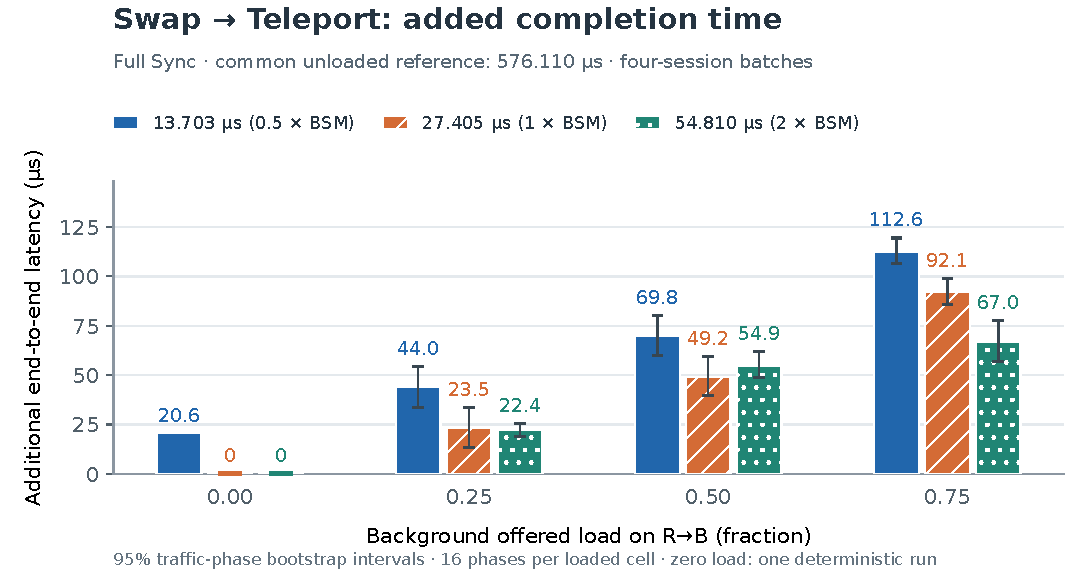
\includegraphics[width=.96\textwidth]{figures/fig1_chain_latency.pdf}
\caption{Additional Full Sync swapping-assisted teleportation latency
above the common unloaded, noncontending reference (576.110~$\mu$s).
Absolute latency is measured from local session start to usable output.
Each group holds network load fixed and
compares the three start intervals. Error bars resample traffic phases;
the zero-load result is deterministic.}
\label{fig:qucl-chain}
\end{figure*}
Figure~\ref{fig:qucl-chain} includes the R swapping queue, result delivery,
B correction, B--R--A readiness, A teleportation queue, A--R--B result
delivery and final B correction. The operation timing and generated
packets are recomputed for every condition.
For half- versus full-service start intervals, the R completion sequence
is identical: the 20.553-$\mu$s difference in mean latency follows from
the different request origins and FIFO waiting. The paired No-R ablation
below specifically changes packet-generation times to test downstream
timing dependence.

\subsection{Simplification Error}
\begin{figure*}[t]
\centering
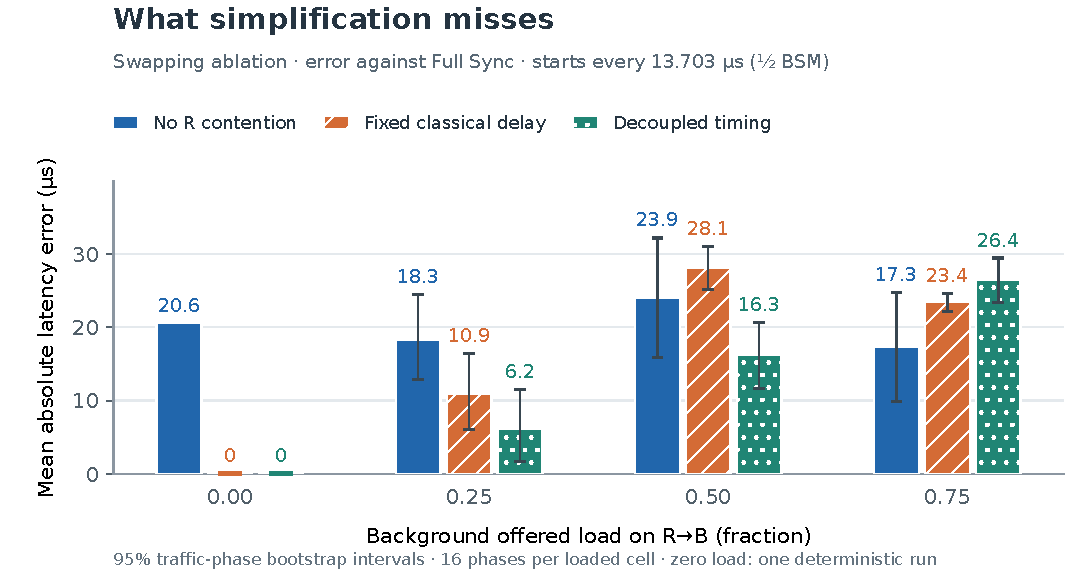
\includegraphics[width=.96\textwidth]{figures/fig2_model_error.pdf}
\caption{Mean absolute latency error against Full Sync for the swapping
ablation at a 13.703-$\mu$s start interval. These are paired protocol-stage
comparisons, not a counterfactual model of the complete chain.}
\label{fig:qucl-models}
\end{figure*}
No R contention removes the R execution-capacity constraint and generates
real packets at the resulting completion times. Fixed classical delay
preserves the R queue but uses its separately calibrated result delay.
Decoupled timing combines No-R result delays with the resource-eligible
FIFO wait. It makes latency predictions only.

At background load 0.75, the latency MAEs for No R contention, Fixed classical delay and Decoupled timing are 17.28, 23.40, 26.44~$\mu$s, respectively (Fig.~\ref{fig:qucl-models}). At zero load, Fixed and Decoupled are exact, while removing R contention yields a 20.553-$\mu$s MAE.

For every paired transaction, the Decoupled latency error equals the
change in result-path delay between No-R and Full Sync. Removing quantum
waiting shifts packet generation relative to background traffic; hence
independently reusing a measured classical delay need not preserve
completion timing. This is a conditional causal counterfactual, not a
claim that load and fidelity must be monotone.

The adopted one-second $T_2$ and microsecond-scale gates also make the
incremental storage-noise effect smaller than under our earlier
illustrative profile. We report branch-weighted fidelity biases in the
artifact and do not interpret differences between physical profiles as
simulator improvements. The retained $F_{\min}=0.5$, 5-ms deadline is an
audit threshold, not a tuned service-failure endpoint.

\paragraph{Scope.}
These results characterize finite four-session batches with randomized
periodic traffic phase, fixed resource-delivery times and a nominal
processor. They do not establish calibrated hardware performance,
steady-state queueing, arbitrary topology scaling, or calibration-free
error bounds. Zero observed errors do not establish zero population error.
